%%% Ch.3: Methodology %%%
\chapter{Methodology and Implementation} \label{ch:method}
The problem of measuring the trustworthiness of communicating entities is an
essential aspect of any online system where they interact with each other for
any purpose, be it shopping, content delivery or file sharing. This chapter
follows on a discussion of a proposed endorsement network where physically or
digitally acquainted entities can endorse each other or their presented
information. The model will address several concerns such as the roles and
requirements of participants as endorser and endorsee, why a participant would
play by the rule and what is to stop them from not doing so, threat models,
etc. With a system of smart contracts, PoC design will confer interaction
between entities, aggregation of information and assignment of scores for final
computation. The storage of data both on and off-chain will be discussed.  

\section{Problem Statement}
To be able to rely on the trustworthiness of an entity as presented by any
online systems, the underlying reputation system needs to be robust and as
transparent as possible. The assurance that available information has not been
tampered with and correctness of claimed identity should be provided to sustain
minimal risk of fraud. The immutable, trustless, decentralized and distributed
attribute of blockchain protocol is a recommended solution on a public
permissionless network.

\section{ User stories \& Requirements} \label{ch:UserStories}
Anyone can join the network and become a participant in the endorsement system.
The two notable roles of a user are endorser and endorsee. An endorser can
initiate the transaction by sending an endorsement to the participant they wish
to. The same user can assume both the roles of endorser and endorsee as long as
a set of predefined requirements are met.  \\ 

%figure - System Context Diagram
\begin{figure}
	\centering
	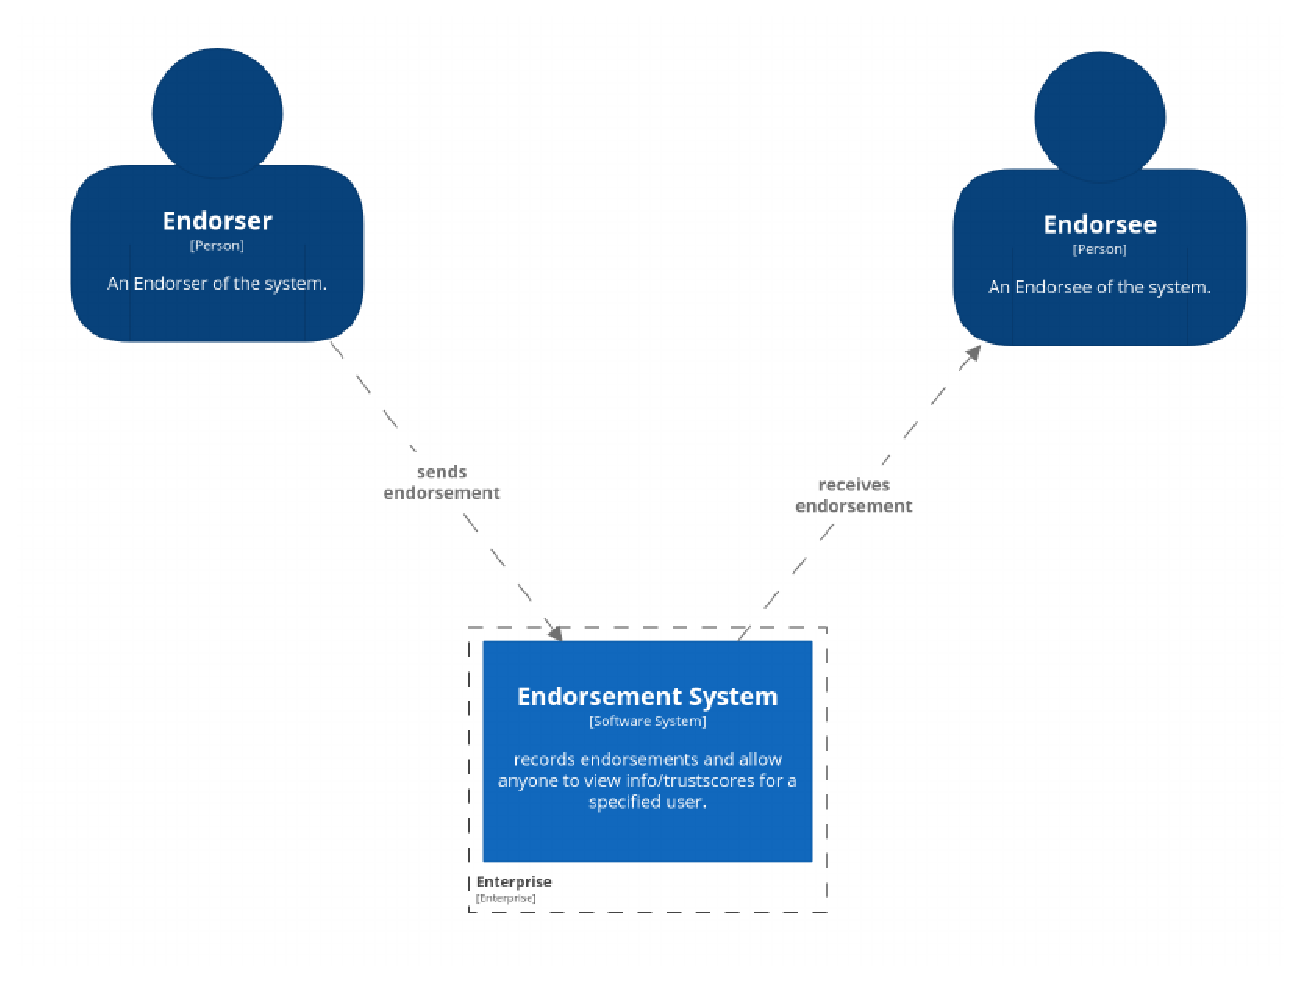
\includegraphics[width=0.8\textwidth]{Images/1SystemContext.eps}
	\caption{Context Layer}
	\label{fig:context}
\end{figure}

The user stories for each role that defines the system requirements for each
user type is presented in table ~\ref{table:userstories}. 
\begin{center} \label{table:userstories}
	\begin{tabular} {| l | p{9cm} | l |}
		\hline
		\textbf{As an}  & \textbf{I need to be able to..}   & \textbf{Traceability} \\
		\hline
		\multirow{2}{*}{Endorser} & send an endorsement so that the endorsement
		is received by the endorsee.& R1
		\\\cline{2-3} 
		& remove endorsement so that the endorsement is removed from the
		endorsee.  & R2 \\\cline{2-3}
		& view a list of endorsees so that i can see to whom i have sent
		endorsements.& R3 \\\cline{2-3}
		& view/edit my personal information so that i can keep it up to
		date& R5 \\\cline{2-3}
		\hline
		\multirow{2}{*}{Endorsee} & view a list of endorsers so that I can see
		from whom I have received endorsements.& R3 \\\cline{2-3}
		\hline
		\multirow{2}{*}{other users} & compute the total endorsement
		impact(i.e., final computed score) of any registered members so that I
		can make an informed decision about the future transactions.
		& R4 \\\cline{2-3}
		& make a request to join the endorsement network so that I can start
		sending/receiving endorsements.  
		& R1 \\\cline{2-3}
		\hline
	\end{tabular}
\end{center}

The functional requirements can be listed in points as : \\
\begin{enumerate}
	\item It must be impossible to make an Endorsement if the endorser and
		endorsee is same address or not a registered participant.
	\item It must be impossible to remove an endorsement if the endorser
		doesn't belong to the list of endorsers for the given endorsee.
	\item All the endorsements must be stored such that, it is possible to see: 
		\begin{itemize}
			\item endorser and endorsee for the given endorsement.
			\item degree of incoming and outgoing connections for all endorsers and endorsees.
		\end{itemize}
	\item There must be a way to link the public key hashes to the
		corresponding computed trust scores. 
	\item It must be possible for a participant to edit their own profile if
		the editor is the same as the profile owner. 
\end{enumerate}

The non-functional system requirements are : \\
\begin{enumerate}
	\item Security: smartcontract security.  
	\item Reliability: reliability of data, tamperproof and verifiable,immutable traceability.
\end{enumerate}

\section{The Model - Endorsement Network}
The initial assumption is that all nodes are honest and as such receive equal
points that they can spend at will once registered on the network. This received
points are the consumable power that keeps depleting with every endorsement
connection made along the way. As depicted in figure ~\ref{consumablePoint} ,
these points follow a convergent sequence that converges to the limit 0 as the
number of connection `n' increases. As such, increasing the number of
connection alone will not be enough to achieve a higher impact on the network.
\begin{figure}
	\centering
	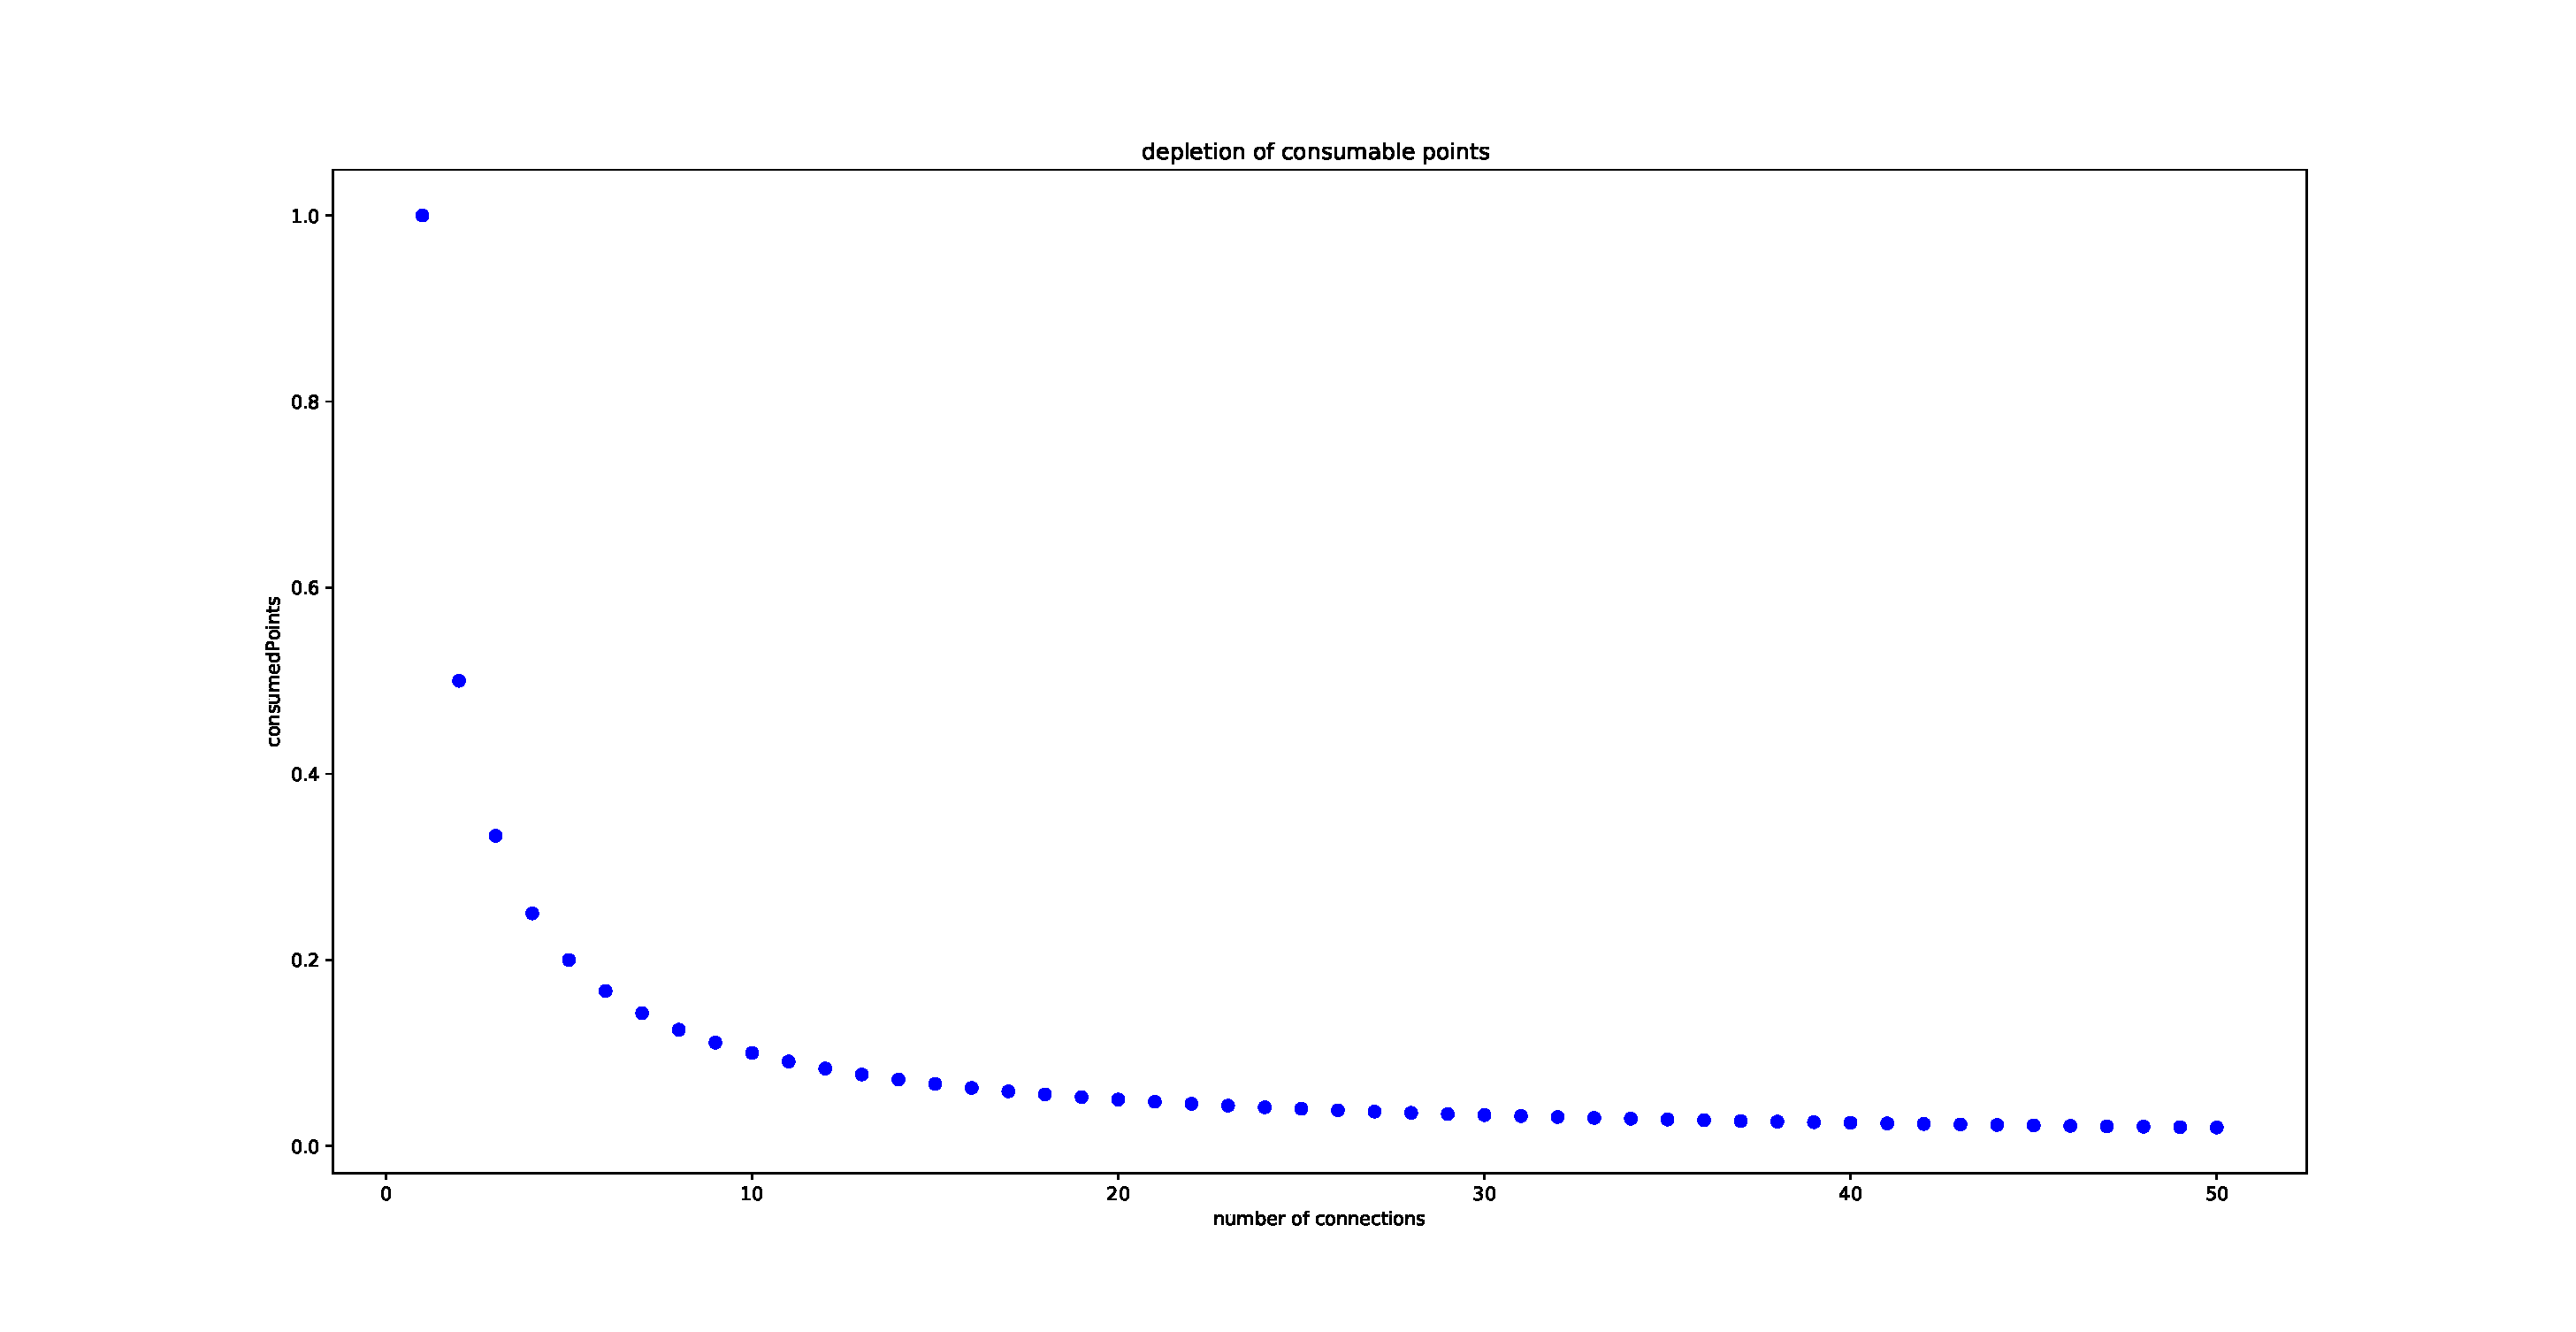
\includegraphics[width=1.0\textwidth]{Images/ConsumablePoints.eps}
	\caption{Convergent behaviour of consumable points as 'n' increases}
	\label{consumablePoint}
\end{figure}

\subsection{Computation of Total Endorsement Impact(tei)} 
The total endorsement impact corresponds to the total impact a participant has
made on the network by sending or receiving endorsements. The two factors that
are primarily responsible for computation of final trust score of a participant
are the number of incoming and outgoing connections. \\

The final trust score, associated with the total endorsement impact a
participant/node has made on the network requires familiarity with some new
terminologies which is briefly discussed below. \\

\textit{$nEG_A$}: number of endorsements sent by a participant 'A'. \\

\textit{$nER_A$}: number of endorsements received by a participant 'A'. \\

\textit{$ratio_A$}: ratio of \textit{$nEG_A$} to \textit{$nER_A$}. This value
ensures that sent and received endorsement are not far off from  each other.
\textit{$ratio_A$} is always assumed to be less than 1 and is given by: 
\begin{equation}
	ratio_A = \frac{min(nEG_A,nER_A)}{max(nEG_A,nER_A)} 
\end{equation}

\textit{$cp_A$}: Total amounts of points spent by a participant 'A' out of the
initially received consumable points. 1 being the initial consumable points
received by everyone who joins the network, \textit{$cp_A$} is given by
1/\textit{$nEG_A$}.

\textit{$TRP_A$}: This corresponds to A's total received points which is the
accumulated sum of consumed points by all endorser of A.  If a peer 'A'
receives an endorsement from 'n' number of peers, then the \textit{$TRP_A$} is
calculated as:
\begin{equation}
	TRP_A  = \sum_{i=0}^{n}cp_{i}
\end{equation}

Finally, the total endorsement impact made by 'A' is given by: \\
\begin{equation}
	TEI_a = ratio_a * cp_a * TRP_a
\end{equation}

%
%ratio of nEG and nER to create a balance in the network
%final score considers both given and received, and how much impact endorser of
%an endorsee has made already

\section{Design of PoC}
This chapter focuses on overview and design details of PoC based on the
requirements mentioned in section \ref{ch:UserStories} on page
\pageref{ch:UserStories}. It starts with design considerations, smart contract
setup, data storage on and off blockchain. The high level system overview is
presented in ~\ref{fig:SystemContainer} 

\begin{figure}
	\centering
	\includegraphics[width=1.3\textwidth]{Images/2Container.eps}
	\caption{Container Layer}
	\label{fig:SystemContainer}
\end{figure}

%\subsection{Formalization}
%The endorsement network as a distributed system can be formally defined by : 
%
%\begin{itemize}
%	\item{P: set of participants $\{p_1,p_2,.. ..,p_j\}$ where 'j' is the total
%		number of participants.} 
%	\item{endorse(x,y): x has sent endorsement to y where $x,y \in P$}
%	\item{receive(y,x): y has received endorsement where $x,y \in P$ }
%	\item{Each participant 'p' has a set of endorsers $\{e_1,e_2,.. ..,e_m\}$
%		and a set of endorsees $\{r_1,r_2,.. ..,r_n\}$ if endorse(e,r) and
%		receive(r,e) is true. Here, 'm'is $nEG_p$	and 'n' is $nER_p$.}
%\end{itemize}

\subsection{Design Consideration}
Honest and malicious participation in the network and the possible behavior
that can result from the interaction between nodes were considered during the
design. From a game-theoretic perspective of a behavioral outcome, following
definition were made for network influencing factors. 

\begin{enumerate}
	\item \label{item:fakeeds} \textbf{Fake endorsements with pseudonymous
		identities:}Endorsement system being on a
		distributed, public permissionless blockchain network allows anyone to
		join and start sending endorsements immediately to whoever they wish
		to. This creates the possibility that an entity could create multiple
		pseudonymous identities with an aim to inflate their impact on the
		network by increasing nEG or nER for their associated persona.  There
		is no straightforward way to detect and stop this behavior right away.
		However, if doing so doesn't provide any significant advantage, then
		the assumption is that a rational decision would be not to do it.  One
		factor that is believed to stop a participant from making too many
		endorsements is the convergent behavior of consumable points. While,
		there is no limit to the amount of connection a participant can form,
		as the number of connection increases, the value of consumable points
		decreases. 
	\item \textbf{Transaction cost:} Ethereum is a programmable blockchain that
		supports a Turing complete programming language. Thus, to avoid running
		in infinite loops or DDOS attacks, gas was introduced. Every operation
		has a gas cost. One could write a program to do anything they wish to
		do on the network as long as the account that initiates the transaction
		can pay the gas cost of all operations. The gas consumption is an
		imperative aspect of endorsement system for two reasons. \\
		\begin{itemize}
			\item \textit{Standard transactions on Ethereum:} A participant
				that makes a call to 'sendEndorsement' function is responsible
				for paying all the required gas costs. This function updates
				the state variable nEG and nER. While the price may not seem
				too high for making one transaction, a malicious node with
				multiple pseudonymous identities has to pay for all the
				operations initiated by all personas. For instance, given the
				interaction graph in the figure, if Alice is an honest node,
				then she only needs to pay for the operation of one
				transaction. Whereas if both Bob and Charlie are the
				pseudonymous identities of Alice, she needs to pay for six
				transactions. Thus, the assumption is that they may make ether
				transfer at some point between their accounts. This information
				is publicly available for anyone on the ethereum blockchain
				network to view the chain of ownership.  If some interactions
				in the endorsement network look suspicious, one could look up
				this detail. This method is not guaranteed to detect a Sybil
				node on the endorsement network but is just another additional
				factor that might be useful before making a decision. 
			\item \textit{ Local information of all neighbouring nodes:}
				Whenever an endorser makes a new connection, the nEG, and
				consumable point change accordingly. This change in consumable
				point has to be reflected for the list of all endorsees. This
				is not to be confused with a one time update. Every new
				connection made by an endorser changes the state for all
				his/her old endorsees. Therefore, all the neighboring nodes of
				an endorser should be stored previously. The impact of a
				participant is dependent on his/her direct interaction as well
				as the endorsers(the participants that have endorsed them).
				There is no way to make constant cost lookups and updates for
				this operation. It requires iterating through the list of
				arrays and computing the impact of every endorsee based on the
				updated state variable. While it is possible to iterate 
				through items in the array, the general recommendation is to
				avoid them if possible. One could surely assume that the list
				will not grow too big for two reasons: (a)A rational node will
				not make too many connections for reasons mentioned earlier in
				~\ref{item:fakeeds} (b)Dunbar's number suggests a cognitive
				limit of 150-250 stable social relationships for humans. \\
				One way to approach this problem is to store the list of
				endorsees and endorsers for a participant but not change the
				state. The computation can be done on the client-side using
				language such as javascript. The final score will be done by
				the client. However, all the variables necessary to compute the
				final score will be stored and updated on blockchain as a
				publicly verifiable information.
		\end{itemize}
	\item \textbf{Dynamism:} The dynamic social behavior of human is that trust
		between two entities is not perpetual. Alice may have trusted Bob
		yesterday but refuses to endorse him today. Trust is dynamic and so is
		the endorsement decision that an entity can take. Therefore, the design
		also considers removal of endorsement previously assigned. The removal
		of endorsement is captured by the figure  ~\ref{fig:removeEds}. 
	\item \textbf{Free-Riders Problem:} Free riders problem is addressed by
		making it necessary to maintain the ratio between nEG and nER. A peer
		without a balanced proportion cannot have a significant impact score on
		the endorsement network. This method also discourages Sybil nodes
		because each identity needs to have an almost equal bi-directional
		connection. If they are only receiving from their own pseudo identity
		that don't have too many connections, then the impact is ignorant and
		thus useless and not worth the time.
\end{enumerate}
\begin{figure}
	\centering
	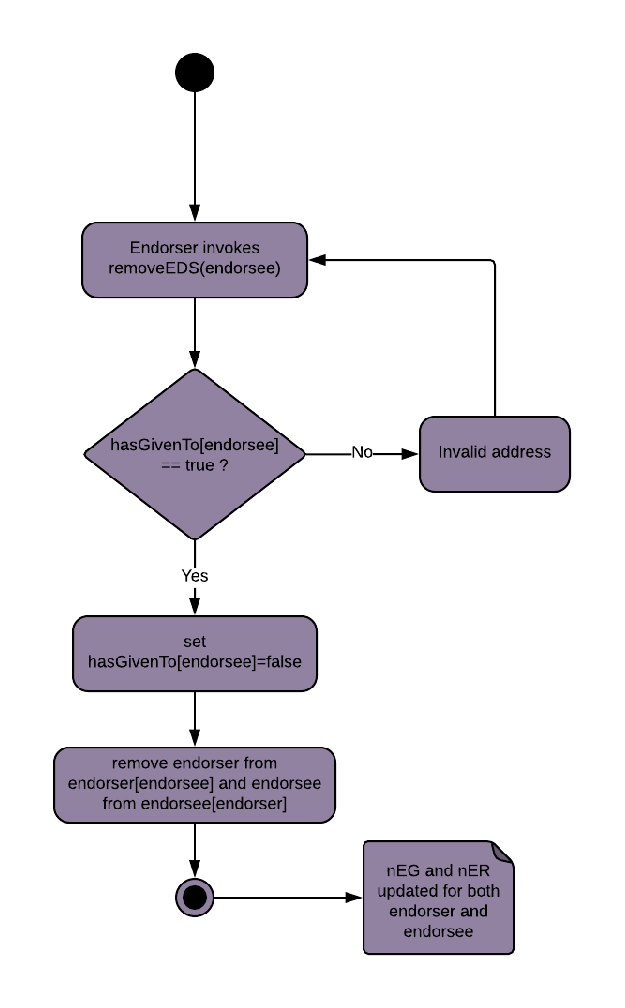
\includegraphics{Images/ActivityDiagramRemoveEDS.eps}
	\caption{Activity diagram for removing endorsement}
	\label{fig:removeEds}
\end{figure}


\subsection{SmartContract} 
The startup process for registering the contract on the public blockchain
network is shown in figure ~\ref{fig:startup}. Smart contracts can be either
deterministic which doesn't require any information from outside blockchain or
non-deterministic which does need to get oracles from external sources.(cite) For
this PoC, endorsement contract is deterministic and so all the data and
variables required are stored and executed on the blockchain.

\begin{figure}
	\centering
	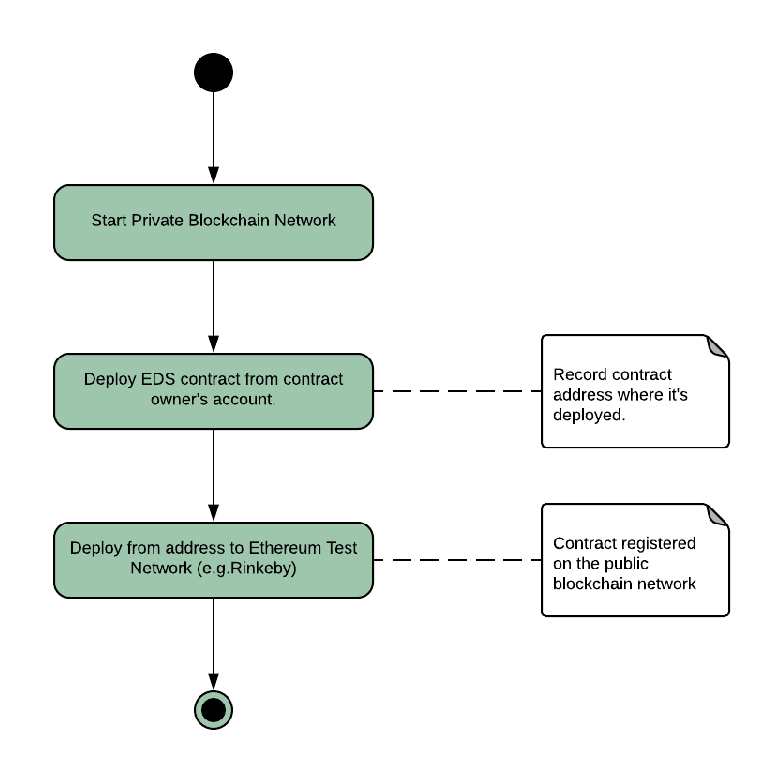
\includegraphics[width=0.8\textwidth]{Images/ActivityDiagramStartUpBC.eps}
	\caption{Startup activity for registering contract on the network}
	\label{fig:startup}
\end{figure}

The system of smart contracts on the component level is depicted in
~\ref{fig:smartcontracts}. The main contracts written for this PoC are : 


\begin{itemize}
	\item Ownable: tracks the owner of the contract. i.e., the creator of
		contract. 
	\item killable: inherits from ownable and can be killed by owner only. 
	\item Participants: set participant and store their information. An index
		to access each participant. 
	\item Endorsement: It inherits from participants and can be called by
		participants only. Endorsement contract handles the core logic of
		endorsement system, accesses/queries addresses from Participants and is
		used for storage of data along with CRUD operations on them.  
	\item Computation: inherits from Endorsement contract and allows anyone to
		get the final score by accessing the current state from an Endorsement
		contract.
	\item Marketplace: stores the buyers, sellers information and allows them
		to buy or sell the product. Also, allows buyer/seller to compute the
		score of the involved entity before doing a transaction.  
\end{itemize}

'Marketplace' contract was written to test the endorsement network on a
transactional network. However, when deploying endorsement system in the real
world, other transactional network/online systems are assumed to have their
reputation platform. The reputation platform should have assigned a score to
the corresponding users based on the behavior on that network. The endorsement
system can act as additional conformity for deciding on a transaction. Say,
Alice is registered on Endorsement network and has made a decent score. If she
wants to sell a product on Marketplace(or any other transactional network), she
can claim about her score and anyone who wants to buy from Alice can verify the
claim by checking the score that corresponds to her public address. If both
Alice and buyer are registered on the endorsement network on the blockchain,
they can send a pre-transaction message to each other to verify that Alice is
who she claims to be and vice-versa. In case the buyer is not registered on the
endorsement network then Alice can prove the claim by signing a cryptographic
challenge with her private key. 

\subsection{Data and variables on and off blockchain}
For this PoC, the data required to identify the users are stored on the
blockchain. But, it does preserve the anonymity requirement mentioned in
section 4.1.1, as the only public information is the link between the public
key hash and individual trust score. Even though the users are required to
register with a pseudonym, it is not needed that the aliases be linked to
real-world identity. A user might like to share more information(other online
account ids, address, etc.).  As mentioned earlier in the gas consumption
section, every non-zero byte data or code of a transaction costs a certain
amount of gas. (cite: eth yellow paper)(cite: eth gas station chart on the gas
section above). Storing this data can become an expensive operation for
real-world usage. The right approach can be to use an off-blockchain storage
solution such as IPFS, swarm (cite). The hash that points to the file in IPFS
can then be stored on the blockchain. Generally, client-side assets (HTML, js)
are stored on these distributed off-chain file system that can communicate to
the contracts registered on blockchain network. 

\begin{figure}
	\centering
	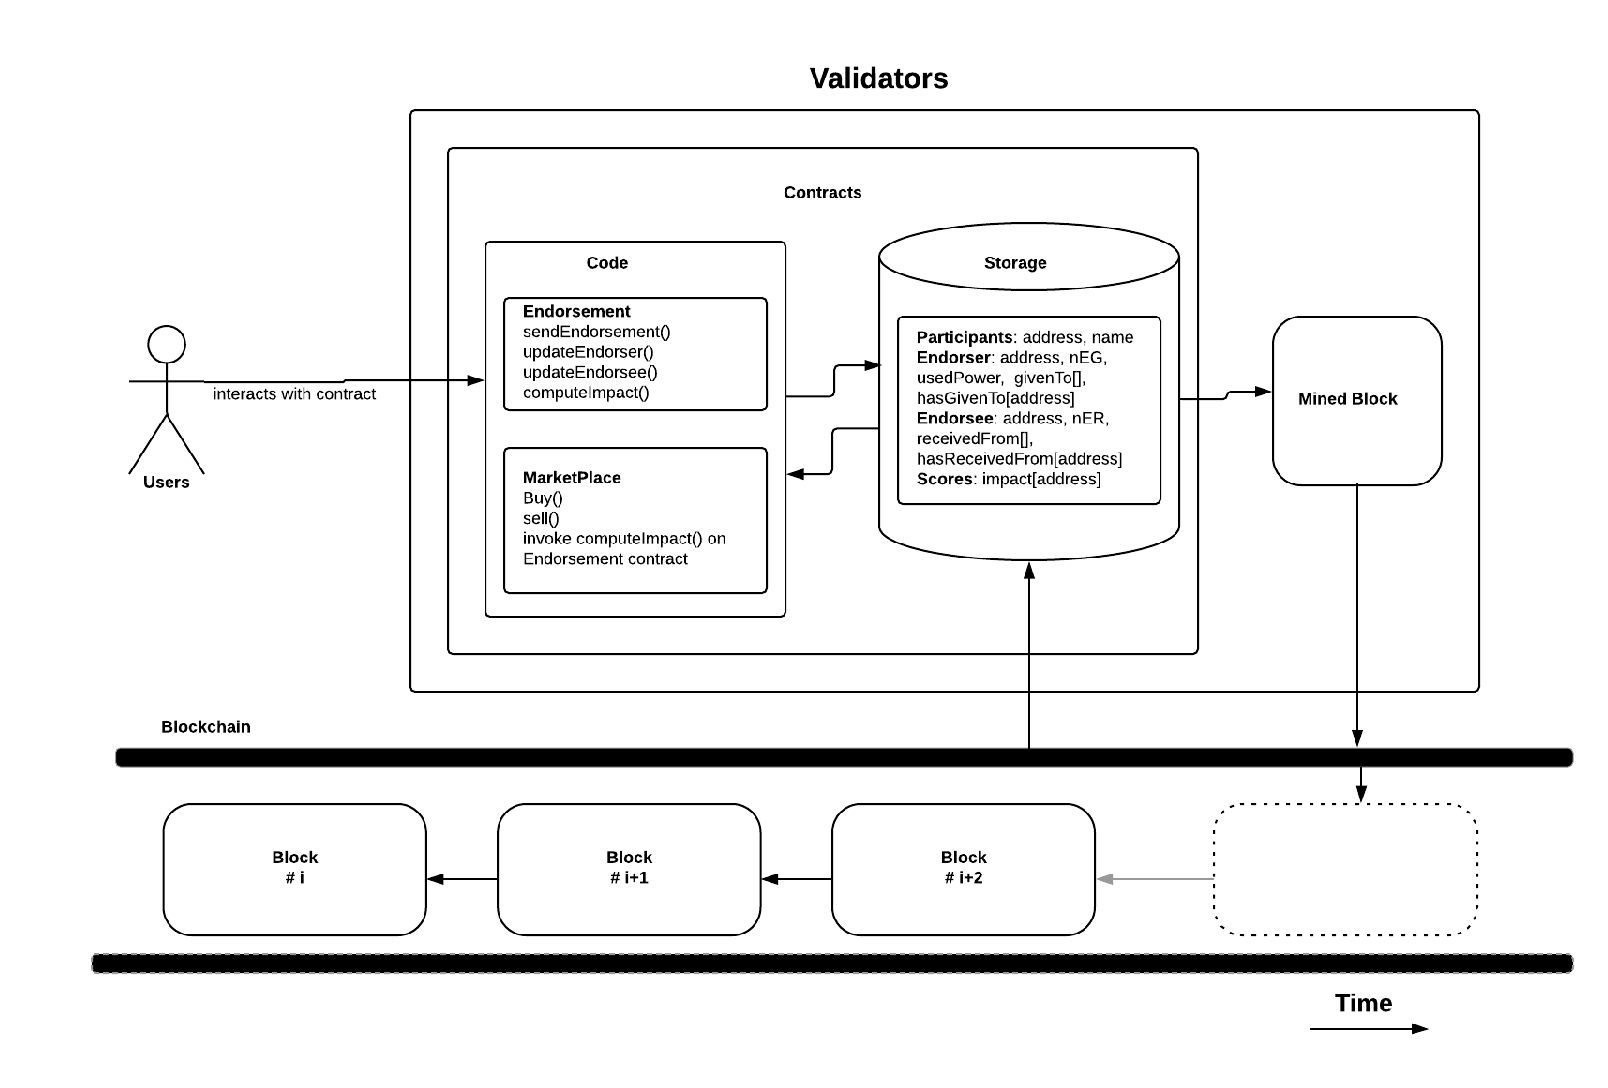
\includegraphics[width=0.8\textwidth]{Images/SmartContractsEDSMarketPlace.eps}
	\caption{Smart contract system}
	\label{fig:smartcontracts}
\end{figure}

\subsection{Blockchain and Consensus algorithms}



%The activity flow of sending an endorsement would look like figure
%~\ref{fig:activity} on page ~\pageref{fig:activity}.

\begin{figure}
	\centering
	\includegraphics[width=0.8\textwidth]{Images/ActivityDiagram.eps}
	\caption{Activity Diagram for sending an endorsement}
	\label{fig:activity}
\end{figure}

%Architecture
%various layers and their communication

%Any registered user can assume both the role of endorser and endorsee. An
%endorser, A must be able to join the network and start sending endorsement
%right away to existing participants in the network. The only requirement for an
%entity to send or receive endorsement is that they both must have joined the
%network before transacting.  The maximum limit is set to 300 for a participant
%to send or receive an endorsement. Based on the definition of Dunbar's number, it
%is the cognitive limit to the number of people one can maintain the social
%relationship with. There is nothing to stop a participant from creating
%multiple identities and endorsing itself but doing so would require twice the
%time which when spent on receiving or sending honest endorsement can be worth
%much more.  The initial points received keeps getting replenished until the
%number hits the maximum limit. The contract also allows for eliminating any
%endorsement previously assigned. Thus, even when a maximum limit is reached,
%users can still actively participate in the network.  Other additional
%requirement includes, A node cannot self-endorse or endorse any node more than
%once. 
%


%\section{Honest vs. Malicious Nodes}
%The 
%
%
%In endorsement network, honest nodes are assumed to endorse only the
%nodes on whom they have full confidence that they will perform the
%fair/legitimate action on the system. In other words, they are ready
%to take the risk if the identities they trusted performs malicious
%activity. It takes time to build a reputation and gain enough trust value
%and therefore giving it all up by endorsing malicious node would not
%be a rational decision. Another assumption is that an honest node will
%have a negligibly low difference between nEG and nER. On the other hand,
%a malicious node will have imbalanced ration between nEG and nER. Using
%the ratio of nEG and nER as one of the metrics may also alleviate the
%common free rider problem discussed earlier.

%User profile : 
% consistent
% declining reputation
% progressing reputation


% The idea is not to exclude malicious behavior in the network, rather include them 
% but give them no value. The endorsement power diminishes every time an entity 
% gives it to someone so the right thing to do for any entity would be to use 
% them wisely. 
% It can be analogous to a gameplay where a player is not restricted to 
% drink a life potion when his lifebar is full but he will waste it if he does with 
% no impact and when the time comes to use it, there won't be any more potion left. 

% Endorsement given (EG) \\
% Endorsement received (ER) \\

% x = 1/EG * ER \\
% y = G:R = no. of people to whom endorsement given : no. of people from whom ends. received \\

% ep = x * y \\ 

% tep = ep * (no. of connection to whom eds given) \\
% drinking potion when you have full life 
% 


%consensus algorithm - 
%what stops someone from making 250 nodes and just endorsing 
%themself.  - net flow rate convergence ,
% would detect this. as we can all 250 nodes are created just to endorse this one 
% node, and so those nodes value would soon converge to zero. 
 
%  It makes no sense to give too much to a node or too less to a node so sybil attack 
%  is almost useless as creating multiple accounts just to endorse someone wont give too 
%  much value. One needs to give/send eds and build trust over time in the network. 
 
%  Problem: What happens if someone plays well in the network for a long time and in 
%  the end decides to betray the whole network. (spy)

% The goal is : once a dishonest node is detected by reputation algorithm in a 
% transaction network, all their endorsement given or received is automatically removed 
% from the network so that will change the values in the dishonest node and other nodes 
% that were connected to it in the past. 

% Question: Modeling this dynamic network and how long it would take or how efficient is it 
% to compute these values within blockchain network? 
% If it makes sense to do the computation in blockchain or off-chain. 
% Only store trust value in the bc network and do other computation elsewhere? 

% net flow rate convergence can also be used to determine anomaly in the network. 

% incentivize honest behaviour.


%Model as interaction graph
%quantify endorsement as reputation score and translate to trust value
%mention reputation algorithm as necessary to be used on the n/w. 




%free rider problem is solved. as given and received balance
%colluding to inflate or damage
% is unanimous with the network and has 
% maximum trust score 
%profile types: progressive, consistent, fluctuating
%Definition and characteristic
%discourage malicious behaviour and encourage honest behaviour
\section{Trust Metrics}

%central nodes, 
%How is trust measured?
%What is required for it to be a correct solution? 
%objective way of accepting or rejecting the work
Every node keeps track of its neighbouring node and whenever an intera



\section{Experimental Setup} \label{sec:sectionlabel}
% 
% 

%Test Network describe, no. of nodes, level of difficulty etc.


%\section{second section}
% It may include: Description of the methodological, theoretical, conceptual or empirical framework; design of the
% experiment; relevant steps of reasoning; data description and sources.

% Describe the approach and method(s) used to address the scientific problem. Also reflect on the particular choice of method and justify it.
